Die Ansätze sollen anhand eines konkreten Beispiels verglichen werden. Hierzu werden die Werte aus \cite{Isemann} Kapitel 11.2.3 verwendet.
Die Parameter des Systems lauten:

\makebox[1cm]{$D$}    = 0.35 m \par
\makebox[1cm]{$\mu$}  = 0.04\par
\makebox[1cm]{$m_1$}  = 2486.7 t\par
\makebox[1cm]{$m_2$}  = 1619.5 t\par
\makebox[1cm]{$R$}    = 2.5 m\par

Es soll ein Antwortspektrum mit folgenden Eckperioden und Bodenbeschleunigung verwendet werden.

\makebox[1cm]{$T_B$}  = 0.4 s\par
\makebox[1cm]{$T_C$}  = 1.6 s\par
\makebox[1cm]{$T_D$}  = 2.0 s\par
\makebox[1cm]{$a_g$}  = 3.924 m/s\textsuperscript{2}\par

\begin{figure}[h]
    \centering
    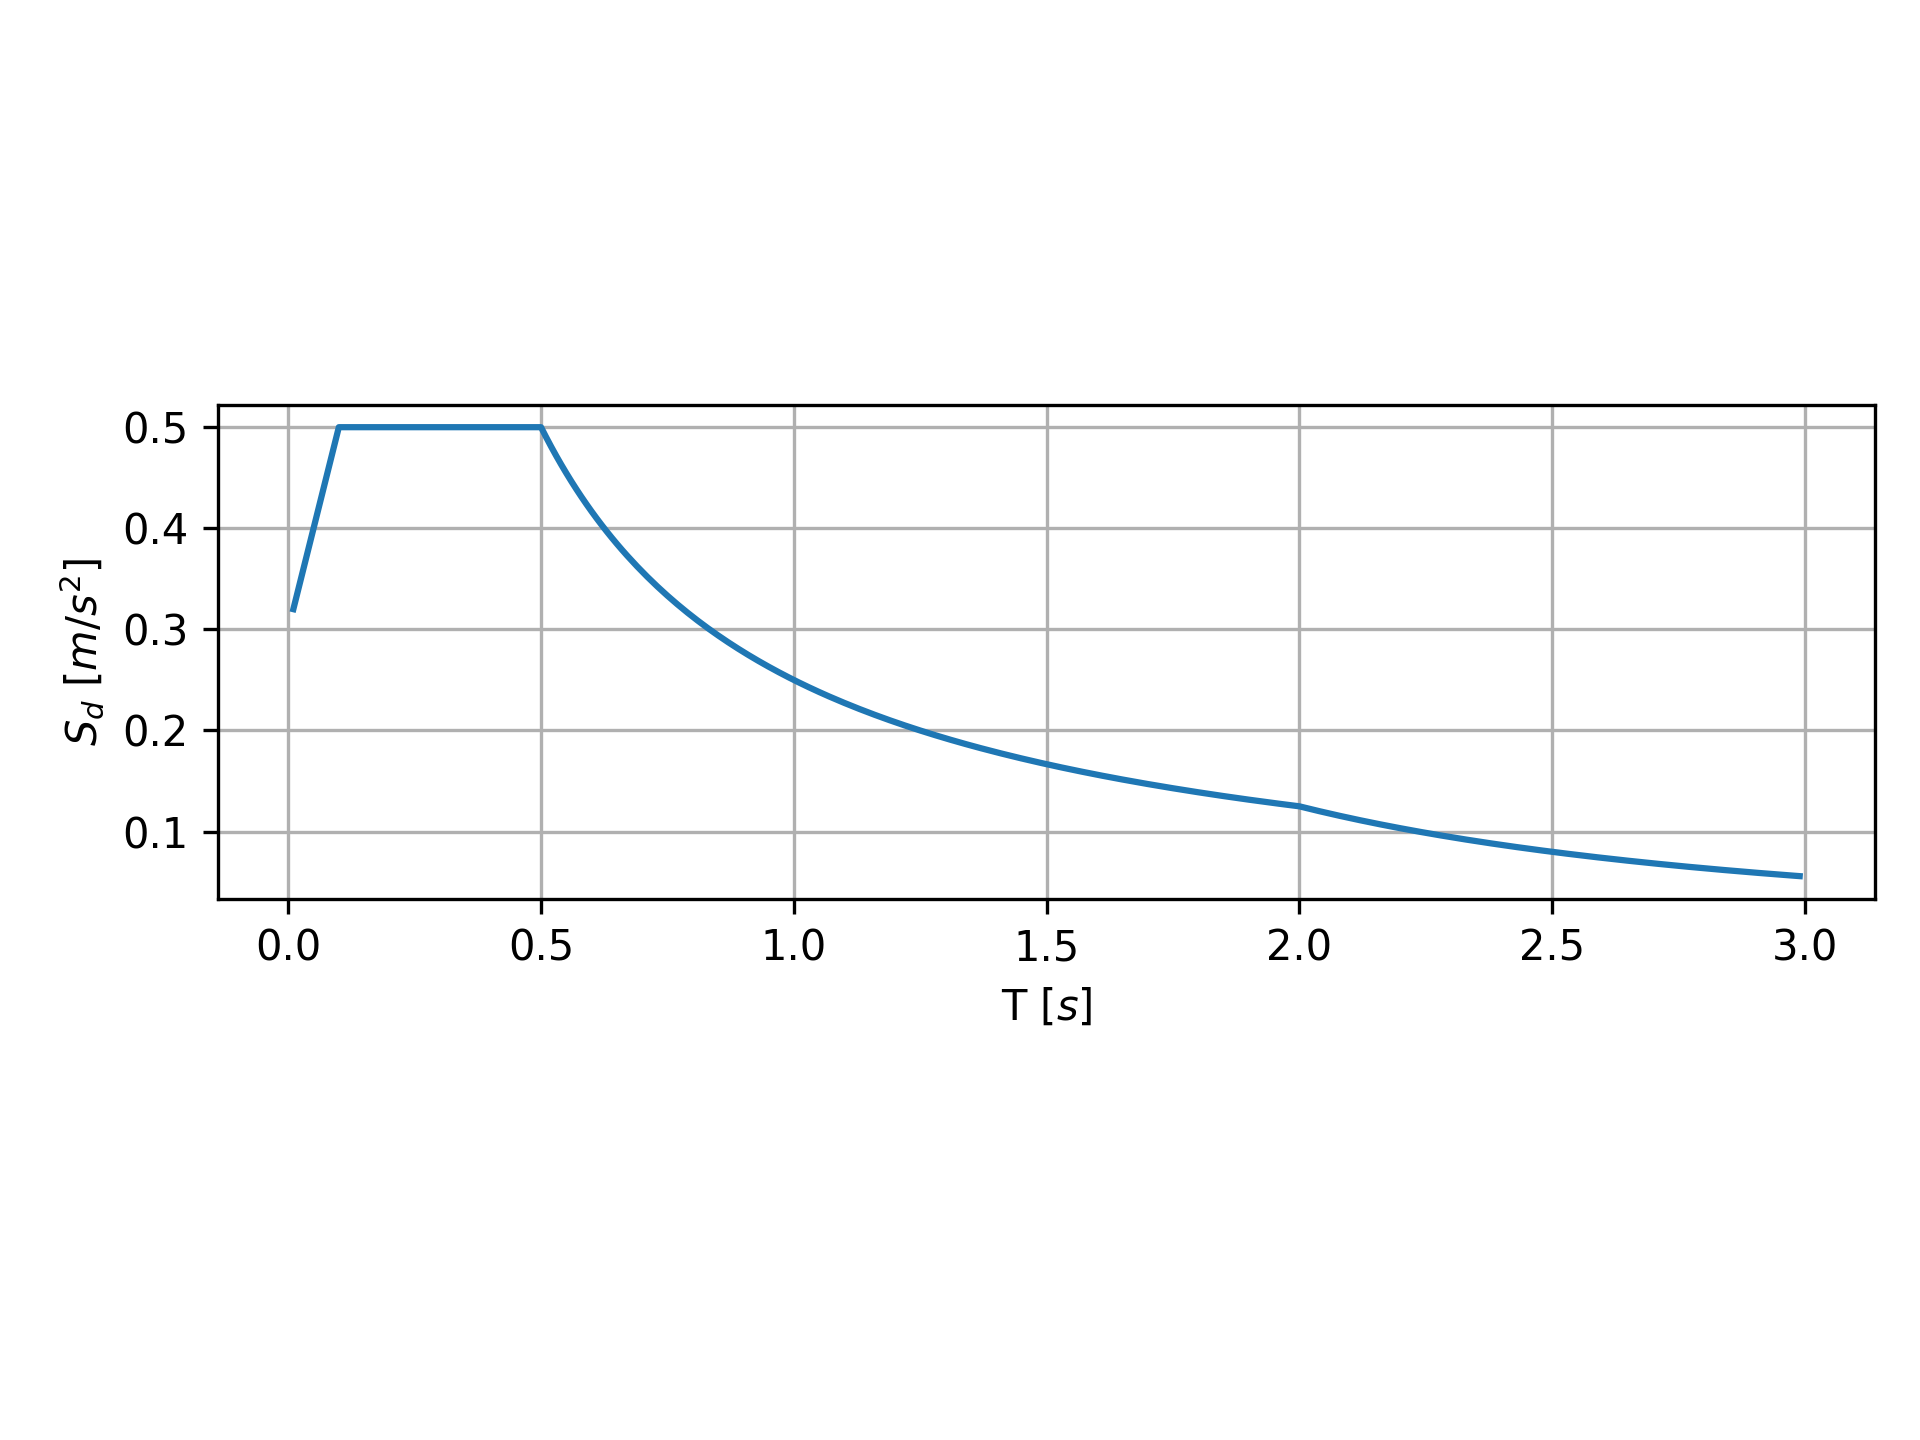
\includegraphics[width=0.9\textwidth]{AWS_beispiel.png}
    \caption{Antwortspektrum (Beispiel 1)}
\end{figure}

Die Steifigkeit $k_2$ ergibt sich aus der effektiven Steifigkeit des Isolators nach \cref{keff}

\begin{equation*}
k_2 = k_{eff} = \frac{G}{R} + \mu \frac{G}{D} = \frac{41062 kN}{2.5 m} + 0.04 \cdot \frac{41062 kN}{0.35 m} = 21117 kN/m
\end{equation*}

Die Dämpfung $\xi_1$ wird mit 5 \% angenommen und die effektive Dämpfung des Isolators $\xi_2$ nach \cref{xieff} bestimmt.

\begin{equation*}
\xi_2 = \xi_{eff} = \frac{2}{\pi} \frac{\mu R}{(D + \mu R)} = \frac{2}{\pi} \frac{0.04 \cdot 2.5 m}{(0.35 m + 0.04 \cdot 2.5 m)} \approx 0.14147
\end{equation*}

\pagebreak

Hier sollen zunächst die Ergebnisse für eine Periode der aufgehenden Struktur von $T = 1 s$ betrachtet werden. Daraus ergibt sich eine Steifigkeit $k_1$ von

\begin{equation*}
k_1 = m_1 (\frac{2 \pi}{T})^2 = 2486.7 t \cdot (\frac{2 \pi}{1 s})^2 = 98170 kN/m
\end{equation*}

\pagebreak

\section{Betrachtung als effektiver Einmassenschwinger}

Wie in \cref{sec:schwierigkeitenvordimensionierung} erwähnt, kann das System unter der Annahme, dass der Isolator die Eigenform dominiert (\cref{Verteilung}), auch als vereinfachter Einmassenschwinger modelliert werden.

Die Eigenperiode beträgt dann

\begin{equation*}
\omega = \sqrt{\frac{k_2}{m_1 + m_2}} = \sqrt{\frac{21117 kN/m}{4106.2 t}} \approx 2.267 \frac{1}{s}
\end{equation*}

\begin{equation*}
T = \frac{2 \pi}{\omega} = \frac{2 \pi}{2.267 \frac{1}{s}} \approx 2.77 s
\end{equation*}

Für eine Periode von $T = 2.77 s$ im Bereich $T_D \leq T$ und unter der Annahme, dass auch die Dämpfung des Isolators dominiert ($\eta=\sqrt{10/(5+14.147)} \approx 0.723$), beträgt die Spektralbeschleunigung

\begin{align*}
S_a(T) &= a_g \eta 2.5 \frac{T_C T_D}{T^2}\\
       &= 3.924 m/s^2 \cdot 0.723 \cdot 2.5 \cdot \frac{1.6 s \cdot 2.0 s}{(2.77 s)^2}\\
       &= \underline{\underline{2.958 m/s^2}}
\end{align*}

\pagebreak

\section{Vereinfachtes Verfahren}

Im ersten Schritt wird die Eigenkreisfrequenz des nicht isolierten Bauwerks $\omega$ und die Verhältniswerte $\alpha$ und $\beta$ ermittelt.

\begin{align*}
\omega &= \sqrt{\frac{k_1}{m_1}} = \sqrt{\frac{98170 kN/m}{2486.7 t}} = 6.2832 \frac{1}{s}\\
\end{align*}

\begin{align*}
\alpha &= \frac{k_2}{k_1} = \frac{21117 kN/m}{98170 kN/m} = 0.2151 & \beta  &= \frac{m_2}{m_1} = \frac{1619.5 t}{2486.7 t} = 0.65\\
\end{align*}

Damit lassen sich die Eigenkreisfrequenzen und Perioden des isolierten Systems bestimmen.

\begin{align*}
\omega_{L,1}^2 &= \frac{1 + \alpha + \beta - \sqrt{(1 + \alpha + \beta)^2 - 4 \alpha \beta}}{2 \beta} \omega^2\\
               &= \frac{1 + 0.215 + 0.65 - \sqrt{(1 + 0.215 + 0.65)^2 - 4 \cdot 0.215 \cdot 0.65}}{2 \cdot 0.65} \cdot (6.2832 \frac{1}{s})^2\\
               &= 4.7504 \Rightarrow  \omega_{L,1} = 2.18 \frac{1}{s}\\
\end{align*}

\begin{align*}
T_{L,1} &= \frac{2 \pi}{\omega_{L,1}} = \frac{2 \pi}{2.18 \frac{1}{s}} = 2.882 s
\end{align*}

Für die Periode von $T = 2.77 s$ im Bereich $T_D \leq T$ und der Dämpfung des Isolators mit $\eta=\sqrt{10/(5+14.147)} \approx 0.723$ beträgt die Spektralbeschleunigung

\begin{align*}
S_a(T) &= a_g \eta 2.5 \frac{T_C T_D}{T^2}\\
       &= 3.924 m/s^2 \cdot 0.723 \cdot 2.5 \cdot \frac{1.6 s \cdot 2.0 s}{(2.882 s)^2}\\
       &= 2.733 m/s^2
\end{align*}

\pagebreak

Um dann die maximale Beschleunigung zu erhalten, wird noch der erste Eigenvektor und Beteiligungsfaktor berücksichtigt.

\begin{align*}
r_1 &= \frac{1 + \alpha - \beta + \sqrt{(1 + \alpha + \beta)^2 - 4 \alpha \beta}}{2} \\
    &= \frac{1 + 0.215 - 0.65 + \sqrt{(1 + 0.215 + 0.65)^2 - 4 \cdot 0.215 \cdot 0.65}}{2}\\
    &= 1.137
\end{align*}

\begin{align*}
\vec{\Phi}_1 &= \binom{1/r_1}{1} = \binom{1/1.137}{1} = \binom{0.8795}{1}
\end{align*}

\begin{equation*}
L_1 = \frac{\vec{\Phi}_1^T M \vec{I}}{\vec{\Phi}_1^T M \vec{\Phi}_1} = \frac{
\begin{pmatrix}
  0.8795 & 1
\end{pmatrix}
\begin{bmatrix}
  1619.5 t & 0 t\\
  0 t & 2486.7 t
\end{bmatrix}
\begin{pmatrix}
  1\\
  1
\end{pmatrix}
}{
\begin{pmatrix}
  0.8795 & 1
\end{pmatrix}
\begin{bmatrix}
  1619.5 t & 0 t\\
  0 t & 2486.7 t
\end{bmatrix}
\begin{pmatrix}
  0.8795 \\
  1
\end{pmatrix}}
= 1.0458
\end{equation*}

\begin{equation*}
\ddot U_{max} = \vec{\Phi}_1 L_1 S_a(T_{L,1}, \xi_{L,1}) = 1.0 \cdot 1.0458 \cdot 2.733 m/s^2 = \underline{\underline{2.858 m/s^2}}
\end{equation*}

\pagebreak

\section{Verfahren der Transmissibilität}

Zunächst werden die Dämpfungsbeiwerte mit dem Ansatz der Rayleigh-Dämpfung ermittelt. Dafür werden die Eigenkreisfrequenzen des ungedämpften Systems benötigt.

\begin{align*}
\omega_{1,2}^2 &= \frac{(k_2 + k_1) m_1 + k_1 m_2 \pm \sqrt{((k_2 + k_1) m_1 + k_1 m_2)^2 - 4 m_2 m_1 k_2 k_1}}{2 m_2 m_1}\\
               \intertext{mit $(k_2 + k_1) m_1 + k_1 m_2 = (21117  + 98170 ) \cdot 2486.7  + 98170  \cdot 1619.5 = 455568212.9 $ \newline und $4 m_2 m_1 k_2 k_1 = 4 \cdot 1619.5  \cdot 2486.7  \cdot 21117  \cdot 98170 = 3.3370719 \cdot 10^{14}$}
               &= \frac{ 455568212.9 \pm \sqrt{((21117  + 98170 ) \cdot 2486.7  + 98170  \cdot 1619.5 )^2 - 3.33.. \cdot 10^{14}}}{2 \cdot 1619.5  \cdot 2486.7 }\\
               &\Rightarrow \omega_1 \approx 2.179 \frac{1}{s}\\
               &\Rightarrow \omega_2 \approx 10.410 \frac{1}{s}
\end{align*}

Damit können die normierten Komponenten der Eigenvektoren bestimmt werden.

\begin{align*}
\varepsilon_1 &= \frac{k_2 + k_1 - m_2 \omega_1^2}{k_1} \\
              &= \frac{21117 kN/m + 98170 kN/m - 1619.5 t \cdot (2.179 \frac{1}{s})^2}{98170 kN/m}\\
              &= 1.136
\end{align*}
\begin{align*}
\varepsilon_2 &= \frac{k_2 + k_1 - m_2 \omega_2^2}{k_1} \\
              &= \frac{21117 kN/m + 98170 kN/m - 1619.5 t \cdot (10.410 \frac{1}{s})^2}{98170 kN/m}\\
              &= -0.572
\end{align*}

\begin{align*}
\varphi_{11} &= \sqrt{\frac{1}{1 + \varepsilon_1^2}} = \sqrt{\frac{1}{1 + 1.136^2}} \approx 0.660\\
\varphi_{21} &= \varepsilon_1 \varphi_{11} = 1.136 \cdot 0.660 \approx 0.750\\
\varphi_{12} &= \sqrt{\frac{1}{1 + \varepsilon_2^2}} = \sqrt{\frac{1}{1 + (-0.572)^2}} \approx 0.867\\
\varphi_{22} &= \varepsilon_2 \varphi_{12} = -0.572 \cdot 0.867 \approx -0.497
\end{align*}

\pagebreak

Die generalisierten Massen und Steifigkeiten sind dann

\begin{align*}
m_2^* &= \varphi_{11}^2 m_2 + \varphi_{21}^2 m_1 = 0.660^2 \cdot 1619.5 t + 0.750^2 \cdot 2486.7 t\\
      &= 2108.3 t\\[2em]
m_1^* &= \varphi_{12}^2 m_2 + \varphi_{22}^2 m_1 = 0.867^2 \cdot 1619.5 t + -0.497^2 \cdot 2486.7 t\\
      &= 1833.8 t\\[2em]
k_2^* &= \varphi_{11}^2 (k_2 + k_1) - 2 \varphi_{21} \varphi_{11} k_1 + \varphi_{21}^2 k_1\\
      &= 0.660^2 \cdot (21117 kN/m +  98170 kN/m) - 2 \cdot 0.750 \cdot 0.660 \cdot 98170 kN/m\\
      &\phantom{{}=1} + 0.750^2 \cdot  98170 kN/m\\
      &= 10013.4 kN/m\\[2em]
k_1^* &= \varphi_{12}^2 (k_2 + k_1) - 2 \varphi_{22} \varphi_{12} k_1 + \varphi_{22}^2 k_1\\
      &= 0.867^2 \cdot (21117 kN/m +  98170 kN/m) - 2 \cdot -0.497 \cdot 0.867 \cdot 98170 kN/m\\
      &\phantom{{}=1} + -0.497^2 \cdot 98170 kN/m\\
      &= 198759.0 kN/m
\end{align*}

und die Eigenkreisfrequenzen der zwei Einmassenschwinger betragen

\begin{align*}
\omega_1^* &= \sqrt{\frac{k_2^*}{m_2^*}} = \sqrt{\frac{10013.4 kN/m}{2108.3 t}}\\
           &= 2.179 \frac{1}{s}
\end{align*}
\begin{align*}
\omega_2^* &= \sqrt{\frac{k_1^*}{m_1^*}} = \sqrt{\frac{198759.0 kN/m}{1833.8 t}}\\
           &= 10.410 \frac{1}{s}
\end{align*}

\pagebreak

Damit ergeben sich die Dämpfungsbeiwerte der Rayleigh-Dämpfung in der Modalform.

\begin{align*}
\alpha &= \frac{2 \omega_1^* \omega_2^* (\xi_2 \omega_2^* - \xi_1 \omega_1^*)}{\omega_2^{*2} - \omega_1^{*2}}\\
       &= \frac{2 \cdot 2.179 \frac{1}{s} \cdot 10.410 \frac{1}{s} \cdot (0.14147 \cdot 10.410 \frac{1}{s} - 0.05 \cdot 2.179 \frac{1}{s})}{(10.410 \frac{1}{s})^2 - (2.179 \frac{1}{s})^2}\\
       &\approx 0.597\\[2em]
\beta  &= \frac{2 (\xi_1 \omega_2^* - \xi_2 \omega_1^*)}{\omega_2^{*2} - \omega_1^{*2}}\\
       &= \frac{2 \cdot (0.05 \cdot 10.410 \frac{1}{s} - 0.14147 \cdot 2.179 \frac{1}{s})}{(10.410 \frac{1}{s})^2 - (2.179 \frac{1}{s})^2}\\
       &\approx 0.004
\end{align*}

\begin{align*}
c_1^* &= \alpha m_1^* + \beta k_1^* = 0.597 \cdot 1833.8 t + 0.004 \cdot 198759.0 kN/m\\
      &\approx 1909.1\\
c_2^* &= \alpha m_2^* + \beta k_2^* = 0.597 \cdot 1833.8 t + 0.004 \cdot 10013.4 kN/m\\
      &\approx 1300.0
\end{align*}

Durch Rücktransformation in die Normalform werden die Komponenten der Dämpfungsmatrix $C$ erhalten.

\begin{align*}
C &= \vec{\Phi}^{-T} C^* \vec{\Phi}^{-1}\\
  &\Rightarrow c_1 = 867538.6\\
  &\Rightarrow c_2 = 334635.2
\end{align*}

Die Eigenfrequenz der ersten, durch den Isolator gesteuerten, Eigenform beträgt dann

\begin{align*}
\omega_{1d} &= \omega_1 \sqrt{1 - \xi_2^2} = 2.179 \frac{1}{s} \cdot \sqrt{1 - 0.14147^2}\\
            &\approx 2.157 \frac{1}{s}\\
T_1         &= \frac{2 \pi}{\omega_{1d}} = \frac{2 \pi}{2.157 \frac{1}{s}}\\
            &\approx 2.912 s
\end{align*}

\pagebreak

Mit der Periode lässt sich bereits $S_a$ aus dem Antwortspektrum (mit $\eta=1$) ermitteln.

\begin{align*}
S_a(T) &= a_g \eta 2.5 \frac{T_C T_D}{T^2}\\
       &= 3.924 m/s^2 \cdot 2.5 \cdot \frac{1.6 s \cdot 2.0 s}{(2.912 s)^2}\\
       &= 3.702 m/s^2
\end{align*}

Die Transmissibilität kann nun mit den Dämpfungsbeiwerten der Rayleigh-Dämpfung bestimmt werden. Dazu werden zuerst die drei komplexwertigen Transmissionskoeffizienten (mit $\omega = \omega_{1d}$) berechnet.

\begin{align*}
X_1 &= \frac{\omega^2 m_1^*}{k_1^* + i \omega c_1^*} = \frac{(2.157 \frac{1}{s})^2 \cdot 1833.8 t}{198759.0kN/m + i \cdot 2.157 \frac{1}{s} \cdot 867538.6}\\
    &\approx 0.0003 - 0.006i\\[2em]
X_2 &= \frac{\omega^2 m_2^*}{k_2^* + i \omega c_2^*} = \frac{(2.157 \frac{1}{s})^2 \cdot 2108.3 t}{10019.4kN/m + i \cdot 2.157 \frac{1}{s} \cdot 334635.2}\\
    &\approx 0.0003 - 0.010i\\[2em]
X_{12} &= \frac{\omega^2 m_1^*}{k_2^* + i \omega c_2^*} = \frac{(2.157 \frac{1}{s})^2 \cdot 1833.8 t}{10019.4kN/m + i \cdot 2.157 \frac{1}{s} \cdot 334635.2}\\
    &\approx 0.0004 - 0.016i
\end{align*}

\begin{align*}
VT &= \left\lvert \frac{1}{(1 - X_1)(1 - X_2) - X_{12}} \right\rvert\\
   &= \left\lvert \frac{1}{(1 - (0.0003 - 0.006i)) \cdot (1 - (0.0003 - 0.010i)) - (0.0004 - 0.016i)} \right\rvert\\
   &\approx 1.0006
\end{align*}

\begin{align*}
S_{a,isoliert} &= S_a \cdot VT = 3.702 m/s^2 \cdot 1.0006\\
               &= \underline{\underline{3.704 m/s^2}}
\end{align*}

\pagebreak

\section{Vergleich der Ergebnisse}

\begin{table}[H]
\centering
\begin{tabular}{ |c|c|c| } 
 \hline
 Einmassenschwinger & Vereinfacht & Transmissibilität\\
 \hline\hline
 2.958 $m/s^2$ & 2.858 $m/s^2$ & 3.704 $m/s^2$\\
 \hline
\end{tabular}
\caption{Vergleich der Beschleunigungen aus den drei Ansätzen (Beispiel 1)}
\end{table}

Es zeigt sich, dass jeder Ansatz leicht andere Werte liefert. Die Streuung beträgt $\approx 22\%$. 
Um einen besseren Einblick zu erhalten, sollen die gesamten Spektren betrachtet werden. Dafür wird $k_1$ in Abhängigkeit von der Periode $T$ variiert. Die Spektren sind in \cref{fig:Isolation} dargestellt und zeigen, dass im interessanten Bereich der Perioden niedriger als die des Isolators eine Isolation grundlegend abgebildet werden konnte.

\begin{figure}[H]
    \centering
    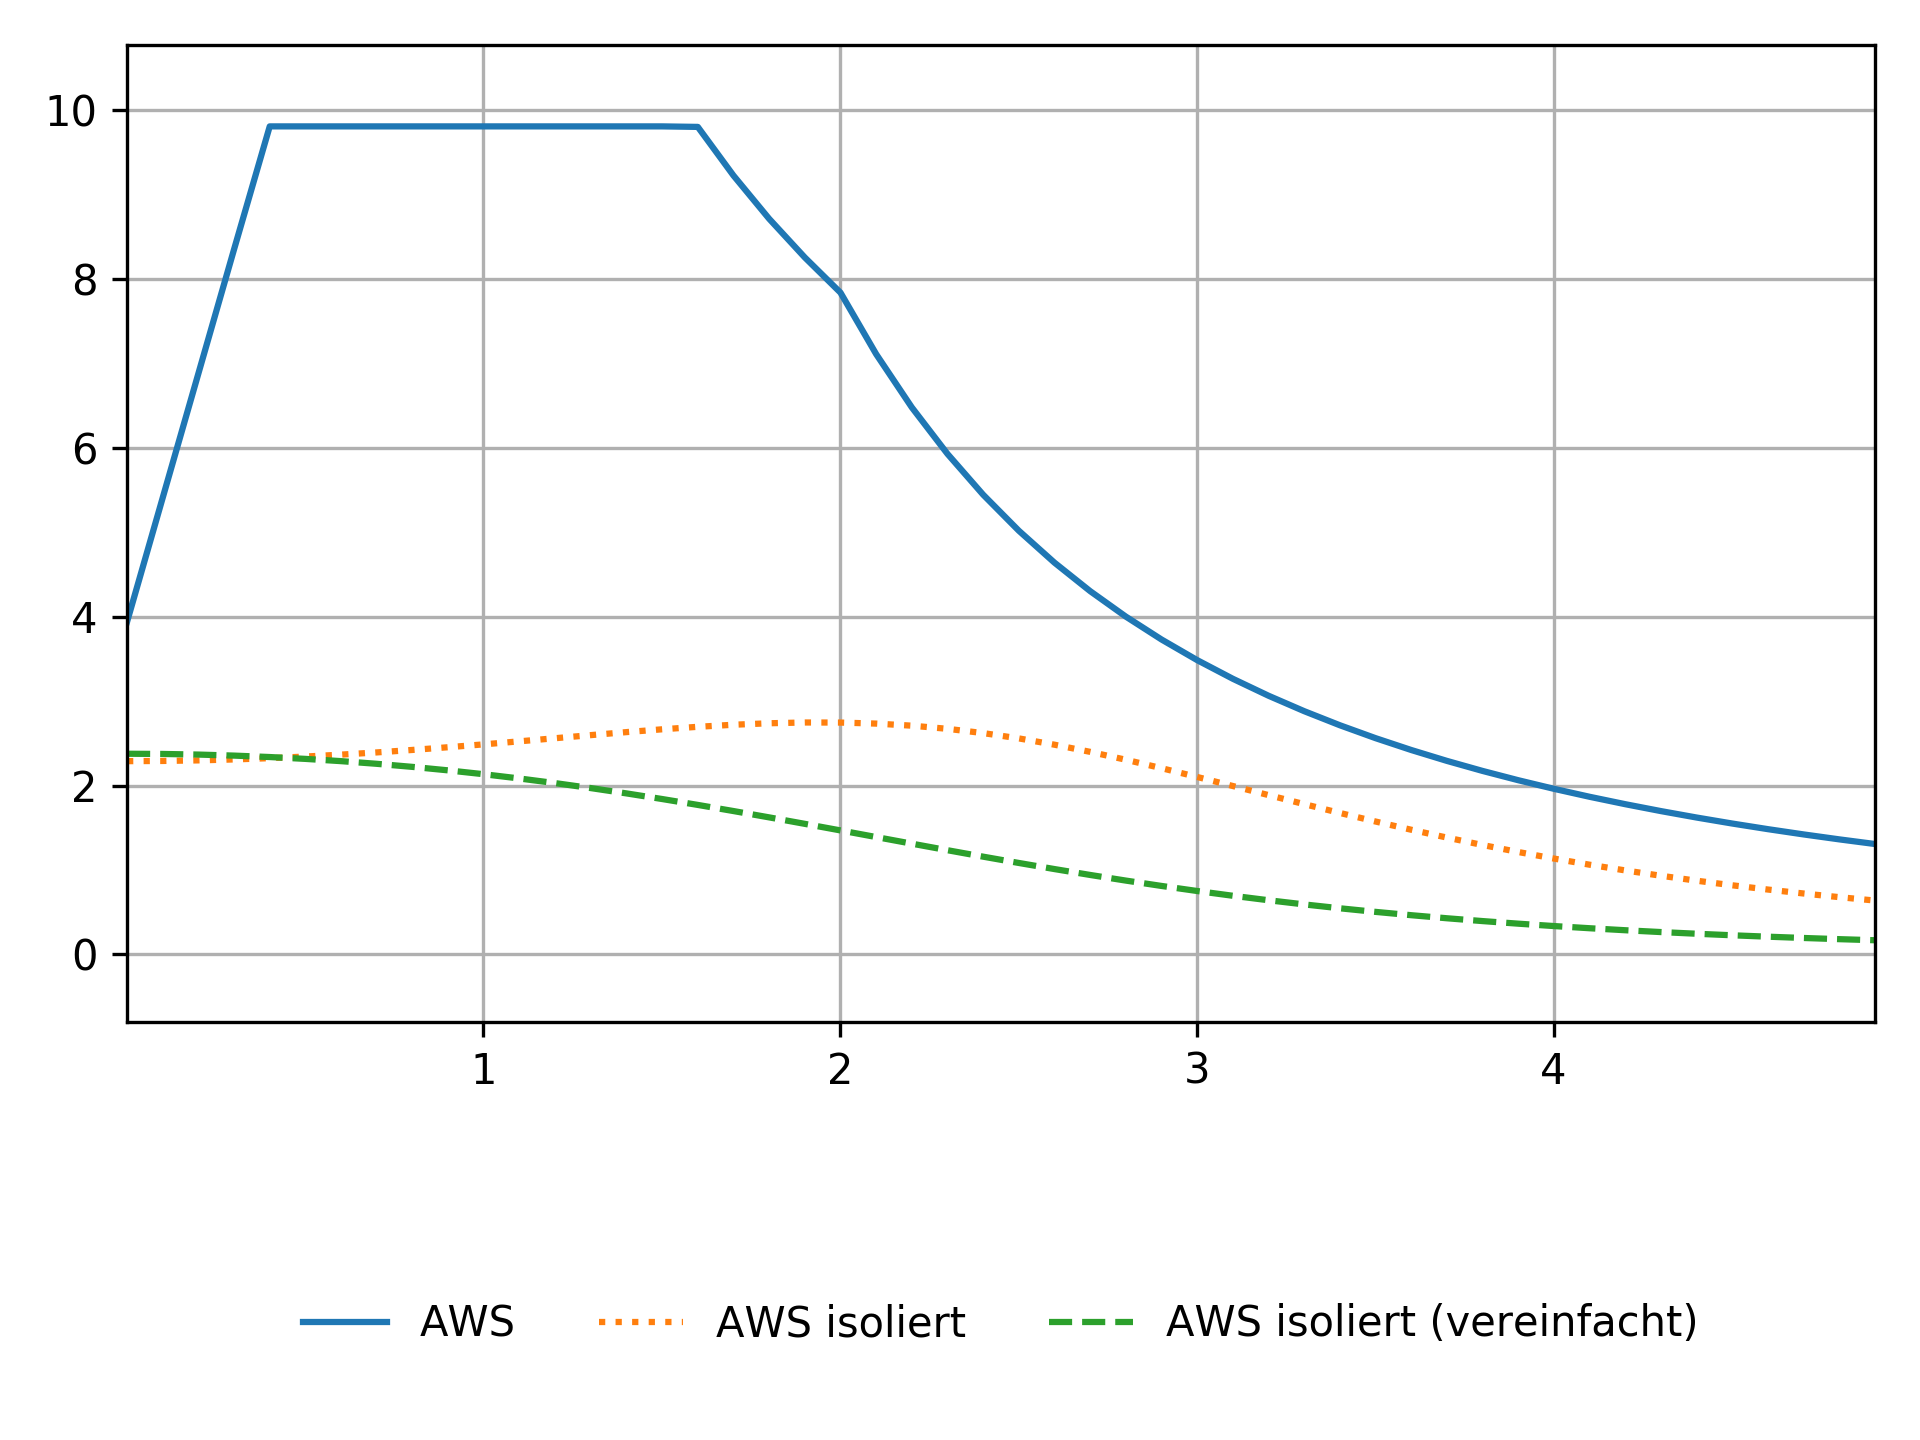
\includegraphics[width=1.0\textwidth]{Isolation.png}
    \caption{Isolationsspektren der drei Ansätze (Beispiel 1)}
    \label{fig:Isolation}
\end{figure}

Wie zu erwarten war, ist die Modellierung als effektiver Einmassenschwinger nur eine Näherung. Die Ergebnisse über die Transmissibilität liefern durchweg größere Beschleunigungen als der vereinfachte Ansatz, wobei sich diese Differenz in der Nähe der Isolatorperiode stärker ausprägt. Auch ist anzumerken, dass die Isolationsspektren geglättet sind, da sie aus dem ebenfalls bereits geglätteten Antwortspektrum berechnet wurden.

\section{Vergleich mit den Ergebnissen einer Zeitschrittberechnung}

Um auch einen Vergleich mit den numerisch ermittelten Werten aus \cite{Isemann} zu machen, wurde das Beispiel in Kapitel 11.3 untersucht.
Mit den angegebenen Massen und der Isolatorsteifigkeit stimmt jedoch die Periode des Isolators, die mit $T = 2.251 s$ angegeben wurde, nicht überein.

\begin{align*}
T &= \frac{2 \pi}{\sqrt{(k_2/(m_2+m_1))}}\\
  &= \frac{2 \pi}{\sqrt{(32000/( 2846.7 t + 1619.5 t)}}\\
  &= 2.347 s \neq 2.251 s
\end{align*}

Die Vermutung liegt nahe, dass für $m_1$ die Masse aus dem vorangegangenen Beispiel in den Berechnungen verwendet wurde und es sich in den Angaben um einen \glqq Zahlendreher\grqq{} handelt.

\begin{align*}
T &= \frac{2 \pi}{\sqrt{(32000/( 2486.7 t + 1619.5 t)}}\\
  &= 2.251 s = 2.251 s
\end{align*}

Mit dieser bestätigten Vermutung wird weiterhin mit $m_1 = 2486.7 t$ gerechnet.
Aus der angegebenen Steifigkeit für den Isolator von $k_2 = 32000 kN/m$ lässt sich der verwendete Radius und das Dämpfungsmaß bestimmen.

\begin{align*}
k_2 &= \frac{G}{R} + \mu \frac{G}{D}\\
    &= \frac{41062 kN}{R} + 0.05 \cdot \frac{41062 kN}{0.325 m} = 32000 kN/m \Rightarrow R \approx 1.599 m
\end{align*}

\begin{equation*}
\xi_2 = \xi_{eff} = \frac{2}{\pi} \frac{\mu R}{(D + \mu R)} = \frac{2}{\pi} \frac{0.05 \cdot 1.599 m}{(0.325 m + 0.05 \cdot 1.599 m)} \approx 0.1257
\end{equation*} 

\pagebreak

Damit stehen die Parameter fest und die Spektren können erzeugt werden.

\makebox[1cm]{$D$}    = 0.325 m \par
\makebox[1cm]{$\mu$}  = 0.05\par
\makebox[1cm]{$m_1$}  = 2486.7 t\par
\makebox[1cm]{$m_2$}  = 1619.5 t\par
\makebox[1cm]{$k_2$}  = 32000 kN/m \par
\makebox[1cm]{$R$}    = 1.599 m\par

\begin{figure}[H]
    \centering
    \includegraphics[width=1.0\textwidth]{_Isolation_2.png}
    \caption{Vergleich der Isolationsspektren aus Zeitschrittberechnung \cite{Isemann}, vereinfachtem Ansatz und Ansatz der Transmissibilität (Beispiel 2)}
    \label{fig:Isolation}
\end{figure}

Hier wird deutlich, dass der vereinfachte Ansatz auf der unsicheren Seite liegt.
Bei dem Ansatz der Transmissibilität liegt die Vermutung nahe, dass die Bestimmung der Beschleunigung am gedämpften Antwortspektrum eine doppelte Berücksichtigung der Dämpfung zufolge hatte, da diese bereits in den Transmissionskoeffizienten erfasst wurde.
Eine Anpassung (\cref{fig:Isolation2}) mit $\eta = \sqrt{10/(5+0)} = 1.4142$ zeigt, dass das Isolationsspektrum nun eine Einhüllende darstellt, allerdings auch deutlich zu große Werte ergibt.

\begin{figure}[H]
    \centering
    \includegraphics[width=1.0\textwidth]{_Isolation_3.png}
    \caption{Vergleich der Isolationsspektren aus Zeitschrittberechnung \cite{Isemann}, vereinfachtem Ansatz und Ansatz der Transmissibilität ($\eta = 1.4142$) (Beispiel 2)}
    \label{fig:Isolation2}
\end{figure}

\section{Korrekturansätze}
\label{sec:Korrekturansaetze}

In \cite{Isemann} wurden verschiedene Ansätze untersucht, das Isolationsspektrum nach oben zu korrigieren.
Auch bei dem Ansatz der Transmissibilität könnte man nun versuchen, die Werte nach unten zu korrigieren. Betrachtet man die Transmissionskoeffizienten (\cref{eq:VT2DOF}), so lässt sich erkennen, dass die Dämpfung auch eine Koppelung darstellt. 

Es soll eine grobe Näherung untersucht werden, nach der die Dämpfungsbeiwerte der beiden Systeme getrennt voneinander bestimmt werden.

\begin{align*}
c_1 &= 2 \xi_1 \sqrt{k_1 m_1}\\
c_2 &= 2 \xi_2 \sqrt{k_2 m_2}
\end{align*}

Die Berechnung der Transmissibilität erfolgt dann am nicht transformierten System.

\begin{equation*}
VT(m_2, k_2, c_2, m_1, k_1, c_1)
\end{equation*} 

\begin{table}[H]
\centering
\begin{tabular}{ |c|c|c| } 
 \hline
 Einmassenschwinger & Vereinfacht & Transmissibilität\\
 \hline\hline
 2.958 $m/s^2$ & 2.858 $m/s^2$ & 3.525 $m/s^2$\\
 \hline
\end{tabular}
\caption{Vergleich der Beschleunigungen aus den drei Ansätzen mit Korrektur (Beispiel 1)}
\end{table}

Die Werte aus dem ersten Beispiel liegen nun deutlich näher zusammen.

\begin{figure}[H]
    \centering
    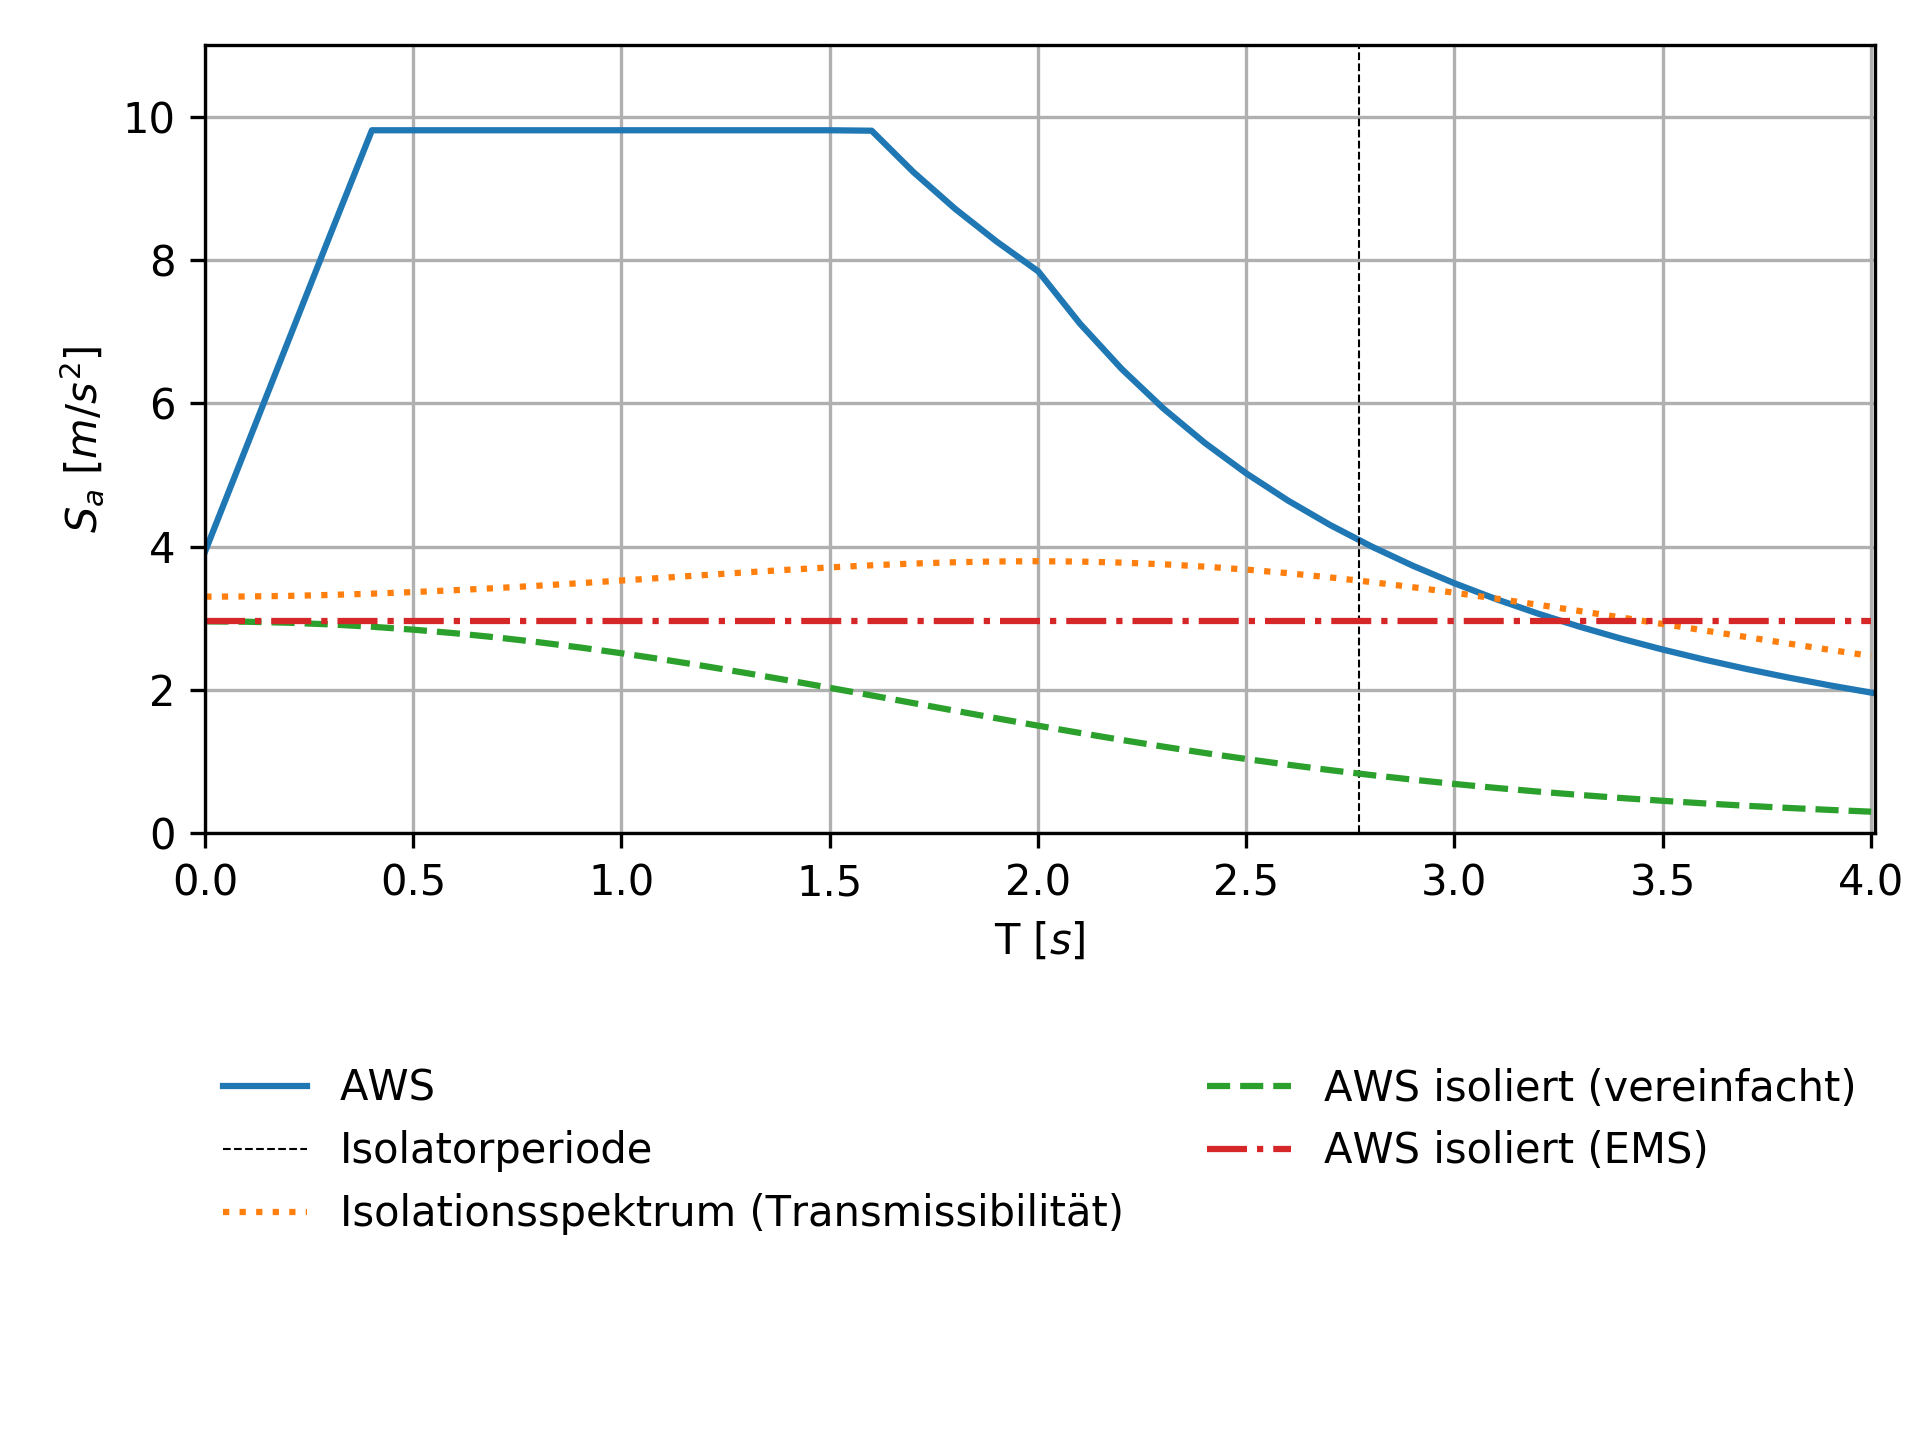
\includegraphics[width=1.0\textwidth]{Isolation_4_2.png}
    \caption{Isolationsspektren der drei Ansätze (Beispiel 1)}
    \label{fig:Isolation2}
\end{figure}


Im zweiten Beispiel (\cref{fig:Isolation21}) kann anhand des Vergleiches der numerisch ermittelten Werte auch festgestellt werden, dass der qualitative Verlauf besser abgebildet werden konnte.

\begin{figure}[H]
    \centering
    \includegraphics[width=1.0\textwidth]{_Isolation_4.png}
    \caption{Vergleich der Isolationsspektren aus Zeitschrittberechnung \cite{Isemann}, vereinfachtem Ansatz und Ansatz der Transmissibilität (Beispiel 2)}
    \label{fig:Isolation21}
\end{figure}

\pagebreak